\section{Função Objetivo}
A função objetivo $f_U$ é definida pela seguinte
expressão:

\begin{dmath}
  f_U = \sum c_i 
\end{dmath}

Onde $\lbrace c_i \rbrace$ é o conjunto formado
por custos e penalizações. Os pesos de cada custo
serão denotados por $p_{descrição}$. São eles:
\begin{enumerate}
  \item Custo da Abertura do Gol
  \item Correção da Abertura do Gol Devido a Movimentação da Bola
  \item Distância Total das Ações $Mover(r)$
  \item Distância Máxima das Ações $Mover(r)$
  \item Mudança do Planejamento da Move Table
  \item Custo do Ataque
  \item Custo das Aberturas vistas por $r \in T_c$
  \item Custo das Aberturas vistas por $r \in T_{ad}$
  \item Custo da Defesa
  \item Número de Receptores
  \item Penalização por Próximidade do Gol do Adversário
  \item Penalização por Proximidade
\end{enumerate}

Além dos parâmetros listados acima, outros parâmetros
afetam o comportamento do time:
\begin{enumerate}
  \item Abertura do gol mínima para chute à gol
  \item Número de ramificações
\end{enumerate}

Esses parâmetros foram os primeiros utilizados no programa.
Ao longo dos testes realizados, foram criados novos parâmetros.
Entretanto, os parâmetros listados são suficientes para ilustrar
a mudança no comportamento do time.

\subsection{Custo da Abertura do Gol}\label{subsec:custo_gap}
O objetivos deste parâmetro é valorizar as aberturas maiores
de acordo com a soma total das aberturas com relação a cada
$r \in T$ e com aberturas maiores.
O cálculo deste custo é feito da seguinte maneira:

\begin{multline} 
 c_{abertura{\ }gol} = taxa_{abertura{\ }total/max{\ }gol} .
   \sum_{r_i \in T} abertura{\ }gol(bola, r)\\
   + (1 - taxa_{abertura{\ }total/max{\ }gol}) .
   max \lbrace abertura{\ }gol(bola, r): r \in T \rbrace 
\end{multline}

As aberturas são calculadas de acordo com a posição de um determinado robô $r$ (obstáculo)
e a posição atual da bola. Isso gera um conjunto de segmentos de reta
$\lbrace abertura{\ }gol(bola, r): r \in T \rbrace$.

Este custo afeta diretamente os seguintes custos:
\begin{itemize}
  \item Custo do Ataque
  \item Custo da Defesa
  \item Custo das aberturas do gol vistas por $r\in T_c$
  \item Custo das aberturas do gol vistas por $r\in T_{ad}$
\end{itemize}

\subsection{Correção da Abertura do Gol Devido a Movimentação da Bola} 
O objetivo deste parâmetro é incorporar a movimentação
da bola pelo atacante no cálculo da abertura do gol. Isso é importante,
pois defensores mais
próximos são mais facilmente driblados que defensores mais distantes. Isso
pode ser visualizado na figura \ref{fig:kick_pos}, onde foi considerada
uma variação de 15cm e de 0cm. Essa variação é medida na linha normal
à reta formada pela bola e pelo robô em questão.

% TODO: Adicionar gráfico detalhado as contas
%       vide arquivo board.cpp para detalhes de implementação

\begin{figure}[H]
  \centering
  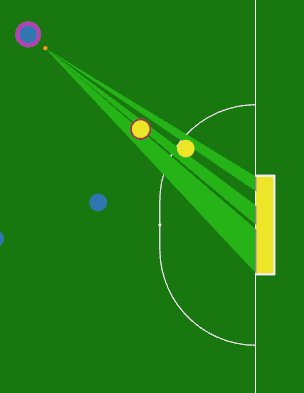
\includegraphics[height=0.4\linewidth]{kick_pos_var_1}
  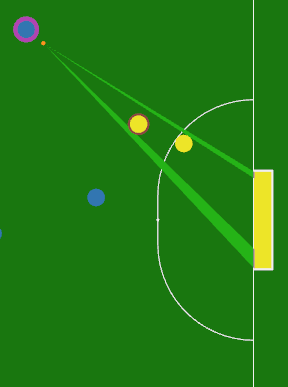
\includegraphics[height=0.4\linewidth]{kick_pos_var_2}
  \caption{Abertura do gol considerando-se uma variação de 15cm na 
           posição da bola (esquerda) e sem variação (direita)}\label{fig:kick_pos}
\end{figure}


\subsection{Distância Total das Ações $Mover(r)$} 
O objetivo deste parâmetro é valorizar o custo da
mudança de estado na função objetivo. Ele é formado pela soma das
distâncias que cada ação $Mover(r)$ irá percorrer partindo das
respectivas posições do estado atual.

\begin{dmath} 
 c_{dist{\ }total{\ }mover} = p_{dist{\ }total{\ }mover} . 
 \sum_{r_i \in T_c} \lVert pos_{r_i} - Mover(r_i)\rVert
\end{dmath} 

\subsection{Distância Máxima das Ações $Mover(r)$} 
O objetivo deste parâmetro é incorporar o custo da
mudança de estado na função objetivo. Ele é formado pela
ação $Mover(r)$ do planejamento atual com maior deslocamento.

\begin{gather} 
 c_{dist{\ }max{\ }mover}= p_{dist{\ }max{\ }mover} . 
 max \lbrace r_i \in T_c : \lVert pos_{r_i} - Mover(r_i)\rVert \rbrace
\end{gather} 

\subsection{Mudança do Planejamento da Tabela de Decisão}\label{subsec:change_cost}
O objetivo deste parâmetro é evitar mudanças grandes no
planejamento da ação $Mover(r)$. Uma das razões para isso é evitar um modelo dinâmico
exato neste nível de planejamento, já que isso aumentaria muito o custo
computacional desta etapa do planejamento e, consequentemente, reduziria
o número de simulações possíveis. Por essas razões mudanças no planejamento
das ações $Mover(r)$ inicialmente foram penalizadas de acordo com a distância euclidiana
entre o $Mover_p(r)$ planejado anteriormente e o $Mover_{m}(r)$ modificado, conforme
a equação:

\begin{dmath} 
 c_{mudança{\ }mover} = p_{mudança{\ }mover} . 
 max \lbrace \sum_{r_i \in T_c} \lVert Mover(r_i) - Mover_p(r_i)\rVert \rbrace
\end{dmath} 

Isso permite que sejam selecionados $Mover_{m}(r)$ mais próximos do
$Mover_p(r)$, refinado assim o planejamento anterior. Entretanto,
um parâmetro mais significativo é o valor absoluto do ângulo entre
essas ações e a posição de $r$, $\lVert ang(r, Mover_{m}(r), Mover_p(r)) \rVert$.
Dessa maneira, tem-se que este custo é computado da seguinte maneira:

\begin{dmath} 
 c_{mudança{\ }mover} = p_{mudança{\ }mover} . 
 max \lbrace \sum_{r_i \in T_c} \lVert ang(r, Mover_{m}(r), Mover_p(r)) \rVert \rbrace
\end{dmath} 

\subsection{Custo do Ataque}
Este custo valoriza situações nas quais o time em questão
possue o domínio da bola (descrito na Subsecção~\ref{subsec:repres_jogo}).

\begin{dmath} 
 c_{ataque} = p_{ataque} . abertura{\ }gol_{ad}
\end{dmath} 

Onde $abertura{\ }gol_{ad}$ é o valor da abertura do gol adversário visto
pelo robô que tem domínio da bola.

\subsection{Custo da Defesa}
Quando não se tem o domínio da bola a abertura do gol do time em questão
visto pelo robô do time adversário que tem a bola é utilizado
como penalização adicional.

\begin{dmath}
  c_{defesa} = p_{defesa} .
   \sum_{r_i \in T_ad} abertura{\ }gol_c(r_i)
\end{dmath}

\subsection{Custo das Aberturas do Gol Vistas por $r\in T_c$}

Este custo tem o objetivo de valorizar configurações nas quais
os robôs que não tem a bola possuam visada para o gol do time
adversário. Isso
é desejavel, já que permite que um gol seja feito caso o robô
que esta com a posse de bola execute um passe para um dos robôs
em questão.

\begin{dmath}
   c_{abertura{\ }gol{\ }ad} = p_{abertura{\ }gol_{ad}} .
    \sum_{r_i \in T_c} abertura{\ }gol_{ad}(r_i)
\end{dmath}

\subsection{Custo das Aberturas do Gol Vistas por $r\in T_{ad}$}

Este custo é o análogo do custo anterior, mas para o
time adversário. Ele visa penalizar situações nas quais
os robôs adversários tenham grande visada (i.e., abertura)
para o gol. 

\begin{dmath}
   c_{bloqueio{\ }gol} = - p_{bloqueio{\ }gol} .
    \sum_{r_i \in T_{ad}} abertura{\ }gol_{ad}(r_i)
\end{dmath}

\subsection{Número de Receptores}

Este custo visa valorizar cituaçõe nas quais existam
vários robôs que possam receber passe.

\begin{dmath}
  c_{receptores} = p_{receptores} .
   num \lbrace r_{receptor_i} \rbrace
\end{dmath}

\subsection{Penalização por Próximidade do Gol do Adversário}
Esta penalização visa evitar que os robôs que estão no ataque
se concentrem dentro da área do time adversário. Caso este
parâmetro não seja adicionado, é esse o comportamento resultante
do custo das aberturas vistas pelos robôs do time em questão. 
A partir de uma determinada distância, é adicionada uma parcela
de penalização na função objetivo.

\begin{dmath}
  c_{penalização{\ }prox} = - p_{penalização{\ }prox}
    \sum num \lbrace r_{perto} \rbrace
\end{dmath}

\subsection{Abertura Mínima para Chute à Gol}
Este parâmetro é o ângulo total da abertura do goal para permitir
o chute pelo atacante. Ele é relevante, pois afeta o comportamento
do atacante e, como consequência, o comportamento do time durante
a posse de bola. Quando a bertura do gol é menor que este valor, o
atacante tem ação de chutar em direção ao goal.

% TODO: Adicionar imagem para ilustrar este caso, já que não tem
%       equações envolvidas

\subsection{Número da Ramificação}
Este parâmetro é o número de possibilidades que serão simulados
em cada iteração do algorítmo de avaliação. Ele influencia o
tempo de resposta do planejamento.
